\section{3. General vector spaces}
% *********************************

\subsection{3.3 Linear independence and basis}
% ============================================

\subsubsection{Exercise 3.3.1}
%-----------------------------

Are the \textbf{A} and \textbf{B} matrices linearly independent?

They are independent if there is no scalar that can multiply one matrix to return the other. So if there
is a solution for $x$  to $Ax = B$, \textbf{A} and \textbf{B} are linearly dependent.

For
$$
\mathbf{A} = \left[\begin{matrix}1 & 1\\1 & 1\end{matrix}\right];
\mathbf{B} = \left[\begin{matrix}2 & 2\\2 & 2\end{matrix}\right];
\mathbf{A}x = \mathbf{B} = \left[\begin{matrix}1 & 1\\1 & 1\end{matrix}\right]x = \left[\begin{matrix}2 & 2\\2 & 2\end{matrix}\right]
$$

$x= 2$ can solve the equation and transform \textbf{A} into \textbf{B} hence the
two matrices are dependent.

\begin{verbatim}
A= Matrix(2, 2, [1,1,1,1])
B= Matrix(2, 2, [2,2,2,2])
solve(Eq(x*A, B), x) # {x: 2} dependent.
\end{verbatim}

The equation $\left[\begin{matrix}1 & 2 \\3  & 4 \end{matrix}\right]x = \left[\begin{matrix}2 & 2\\2 & 2\end{matrix}\right]$
has no solution for $x$, so \textbf{A} and \textbf{B} are independent.

\begin{verbatim}
A= Matrix(2, 2, [1, 2,
                 3, 4])
B= Matrix(2, 2, [2, 2,
                 2, 2])
Eq(A*x, B)
\end{verbatim}

\subsubsection{Example 3.15}
%---------------------------

Given three vectors in the space of continuous functions:

$$
\mathbf{u}= cos(x) \quad
\mathbf{v}= sin(x) \quad
\mathbf{w}= 2
$$

We show they are \textbf{linearly independent} by solving:

$$
k_1\mathbf{u} + k_2\mathbf{v} + k_1\mathbf{w}= 0
$$

For $k_1, k_2, k_3$. If the only solution is for $k_1 = k_2 = k_3 = 0$, the functions
are linearly independent.

To find solutions for $k_1, k_2, k_3$ we need a system of three equations.
In each equation $x$ is replaced by a convenient value which makes the arithmetic
easier. In this case we could use $x= 0, x= \pi, x= \pi/2$. Here we replace $x$ with
a generic constant $c_1, c_2, c_3$ since the dirty job of solving the system is left
to \sympy.

$$
\left[\begin{matrix}
k_{1} \mathbf{u} + k_{2} \mathbf{v} + k_3 \mathbf{w} \\
k_{1} \mathbf{u} + k_{2} \mathbf{v} + k_3 \mathbf{w} \\
k_{1} \mathbf{u} + k_{2} \mathbf{v} + k_3 \mathbf{w} \\
\end{matrix}\right]
=
\left[\begin{matrix}
k_{1} \cos{\left (c_{1} \right )} + k_{2} \sin{\left (c_{1} \right )} + 2 k_{3} \\
k_{1} \cos{\left (c_{2} \right )} + k_{2} \sin{\left (c_{2} \right )} + 2 k_{3} \\
k_{1} \cos{\left (c_{3} \right )} + k_{2} \sin{\left (c_{3} \right )} + 2 k_{3}
\end{matrix}\right]
=
\left[\begin{matrix}
0 \\
0 \\
0 \\
\end{matrix}\right]
$$

\begin{verbatim}
x,k1,k2,k3= symbols('x k1:4', real= True)
u= cos(x)
v= sin(x)
w= 2

eq= Eq(k1*u + k2*v + k3*w, 0)
c1, c2, c3= symbols('c1:4', real= True)
eq1= eq.subs(x, c1)
eq2= eq.subs(x, c2)
eq3= eq.subs(x, c3)
solve([eq1, eq2, eq3], [k1, k2, k3])
\end{verbatim}

Given

$$
\mathbf{f} = \cos^{2}{\left (x \right )}, \quad
\mathbf{g}= \sin^{2}{\left (x \right )}, \quad
\mathbf{h}= 5
$$

The linear combination

$$
k_{1} \mathbf{f} + k_{2} \mathbf{g} + k_3 \mathbf{h} = 
k_{1} \cos^{2}{\left (x \right )} + k_{2} \sin^{2}{\left (x \right )} + 5 k_{3} = 0
$$

is solved with the system

$$
\left[\begin{matrix}
k_{1} \cos^{2}{\left (c_{1} \right )} + k_{2} \sin^{2}{\left (c_{1} \right )} + 5 k_{3} = 0 \\
k_{1} \cos^{2}{\left (c_{2} \right )} + k_{2} \sin^{2}{\left (c_{2} \right )} + 5 k_{3} = 0 \\
k_{1} \cos^{2}{\left (c_{3} \right )} + k_{2} \sin^{2}{\left (c_{3} \right )} + 5 k_{3} = 0
\end{matrix}\right]
$$

where $\left \{ k_{1} : - 5 k_{3}, \quad k_{2} : - 5 k_{3}\right \}$. Since $k_1,
k_2, k_3$ are not all equal to zero, the functions are linearly dependent. 

\begin{verbatim}
f= cos(x)**2
g= sin(x)**2
h= 5

def testLinearIndep(f, g, h):
    ## Linear combination
    k1, k2, k3= symbols('k1:4')
    eq= Eq(k1*f + k2*g + k3*h, 0)
    
    ## Linear system:
    c1, c2, c3= symbols('c1:4')
    eq1= eq.subs(x, c1)
    eq2= eq.subs(x, c2)
    eq3= eq.subs(x, c3)
    
    ## Solutions to linear system
    M= Matrix(3, 1, [eq1, eq2, eq3])
    sols= solve(M, [k1, k2, k3])
    return sols
\end{verbatim}

It can be attcked using Wronskian determinant \textbf{W}. If $\mathbf{W} \neq 0$ 
than the functions are linearly independent. However $\mathbf{W} = 0$ does not
necessarily mean dependence.

\begin{verbatim}
k1, k2, k3= symbols('k1:4')
f= cos(x)**2
g= sin(x)**2
h= 5

def wronskian(f, g, h):
    W= Matrix([[f, g, h],
            [diff(f, x), diff(g, x), diff(h, x)],
            [diff(f, x, 2), diff(g, x, 2), diff(h, x, 2)]])
    return W.det()
    
wronskian(f, g, h) # == 0 => *Suggests* lin. dep.
\end{verbatim}

\subsubsection{Exercise 3.3.3c}
% -----------------------------
\begin{verbatim}
f= 1
g= x
h= x**2
testLinearIndep(f, g, h) #  {k1: 0, k2: 0, k3: 0} => Lin. Indep.
wronskian(f, g, h) # == 2 -> Lin. Indep.
\end{verbatim}

\subsubsection{Exercise 3.3.3d}
% -----------------------------

In this case, the Wronskian appears to be non-zero:

$$
\mathbf{W}= - 3 \sin^{2}{\left (x \right )} \sin{\left (2 x \right )}
\cos{\left (x \right )} - 6 \sin{\left (x \right )} \cos^{2}{\left (x \right )}
\cos{\left (2 x \right )} + 3 \sin{\left (2 x \right )} \cos^{3}{\left (x \right )}
$$

Although it seems to be very close to 0 for any value of $x$.

\begin{verbatim}
f= sin(2*x)
g= sin(x) * cos(x)
h= cos(x)
testLinearIndep(f, g, h) # {k1:-k2/2, k3: 0} => Lin dep.
w= wronskian(f, g, h) # \neq 0. Why?

## Wronskian close to but not zero:
max([float(w.subs(x, c/100)) for c in range(-200*pi, 200*pi)]) # 6.66e-16
\end{verbatim}

\subsubsection{Exercise 3.3.3e}
% -----------------------------

\begin{verbatim}
f= exp(x) * sin(2*x)
g= exp(x) * sin(x)* cos(x)
h= exp(x) * cos(x)
testLinearIndep(f, g, h) # {k1:-k2/2, k3: 0} => Lin dep.
w= wronskian(f, g, h)
max([float(w.subs(x, c/100)) for c in range(-200*pi, 200*pi)]) # 3.818e-08
\end{verbatim}

\subsubsection{Exercise 3.3.3f}
% -----------------------------
\begin{verbatim}
f= 1
g= exp(x)
h= exp(-x)
testLinearIndep(f, g, h) # k1 = k2 = k3 = 0 # Lin. Indep.
wronskian(f, g, h)       # wronskian= 2
\end{verbatim}

\subsubsection{Exercise 3.3.3g}
% -----------------------------

\begin{verbatim}
f= exp(x)
g= exp(2*x)
h= exp(3*x)
testLinearIndep(f, g, h) # k1 = k2 = k3 = 0 # Lin. Indep.
wronskian(f, g, h)       # wronskian == 2*exp(6*x) != 0
\end{verbatim}

\subsubsection{Exercise 3.3.4}
% ----------------------------

Same as exercise 

\begin{verbatim}
f= sin(x)
g= sin(3*x)
h= sin(5*x)
testLinearIndep(f, g, h) # k1 = k2 = k3 = 0 # Lin. Indep.
w= wronskian(f, g, h)  # !=0
\end{verbatim}

\subsubsection{Exercise 3.3.4}
% ----------------------------

Show that the following matrices are a \textbf{basis} for $M_{22}$, the vector space of
2 by 2 matrices.

$$
\mathbf{A}= \left[\begin{matrix}1 & 0\\0 & 0\end{matrix}\right], \quad
\mathbf{B}= \left[\begin{matrix}0 & 1\\0 & 0\end{matrix}\right], \quad
\mathbf{C}= \left[\begin{matrix}0 & 0\\1 & 0\end{matrix}\right], \quad
\mathbf{D}= \left[\begin{matrix}0 & 0\\0 & 1\end{matrix}\right]
$$

The following conditions must satisfied:

\begin{enumerate}
\item \textbf{Span}: Can any vector in $M_{22}$ be generated with \textbf{A, B, C, D}?
\item \textbf{Linear independence}: Are \textbf{A, B, C, D} linearly independent?
\end{enumerate}

To see if \textbf{A, B, C, D} \textbf{span} $M_{22}$ we generate a generic matrix
$\mathbf{M}= \left[\begin{matrix}a & b\\c & d\end{matrix}\right]$ and then we
see if a linear combination of \textbf{A, B, C, D} can produce \textbf{M}:
$$
k_1\mathbf{A} + k_2\mathbf{B} + k_3\mathbf{C} + k_4\mathbf{D} = \mathbf{M}
$$
Yes, we can combine \textbf{A, B, C, D} and produce \textbf{M} by setting
$\left \{ a : k_{1}, \quad b : k_{2}, \quad c : k_{3}, \quad d : k_{4}\right \}$

Are \textbf{A, B, C, D} also linearly independent? In other words is the
linear combination

$$
k_1\mathbf{A} + k_2\mathbf{B} + k_3\mathbf{C} + k_4\mathbf{D} = \mathbf{O}
$$
satisifed for values of $k$s other than $k_1=k_2=k_3=k_4=0$? No, as show in the code.

\begin{verbatim}
A= Matrix(2, 2, [1, 0, 0, 0])
B= Matrix(2, 2, [0, 1, 0, 0])
C= Matrix(2, 2, [0, 0, 1, 0])
D= Matrix(2, 2, [0, 0, 0, 1])

## Span
a,b,c,d= symbols('a b c d')
k1, k2, k3, k4= symbols('k1:5')
M= Matrix(2, 2, [a, b, c, d])
solve(Eq(k1*A + k2*B + k3*C + k4*D, M)) # {a: k1, b: k2, c: k3, d: k4}

## Linear independence
eq= Eq(k1*A + k2*B + k3*C + k4*D, zeros(2,2))
solve(eq) # {k1: 0, k2: 0, k3: 0, k4: 0}
\end{verbatim}

\subsubsection{Exercise 3.3.6}
% ----------------------------

Check whether the three polynomials $p, q, r$ form a basis for the vector space of
the polynomials of degree $\leq 2$.

\begin{enumerate}
\item \textbf{Span}: Take a general polynomial $y$ of degree 2 and see if the linear combination
of the $p, q, r$ can produce $y$
\item \textbf{Linear independence}: Check whether $p, q, r$ are linearly independent.
\end{enumerate}

$p, q, r$ do span $P^2$ by setting
$\left \{ k_{1} : a + b + c, \quad k_{2} : 2 a + b, \quad k_{3} : a\right \}$

$p, q, r$ are linearly independent since the only solution to
$k_{1} + k_{2} \left(t - 1\right) + k_{3} \left(t - 1\right)^{2} = 0$ is for
$\left \{ k_{1} : 0, \quad k_{2} : 0, \quad k_{3} : 0\right \}$.

\begin{verbatim}
t,a,b,c= symbols('t a b c')
k1, k2, k3= symbols('k1:4')
p= 1
q= t - 1
r= (t - 1)**2

## Span
y= a*t**2 + b*t + c
eq= Eq(k1*p + k2*q + k3*r, y)
solve(eq, [k1, k2, k3]) # {k1: a + b + c, k2: 2a + b, k3: a}

## Linear independence
eq= Eq(k1*p + k2*q + k3*r, 0)
solve(eq, [k1, k2, k3]) # {k1: 0, k2: 0, k3: 0}
\end{verbatim}

With $\mathbf{p, q, r}$ we can define any vector in $P^2$. For example, how can we
combine $\mathbf{p, q, r}$ to obtain $\mathbf{p_1} = t^{2} + 1$? \emph{I.e.}, what
coefficients $k_1, k_2, k_3$ do we need to assign to $\mathbf{p, q, r}$? We need to
solve the equation
$$
k_{1}\mathbf{p} + k_{2} \mathbf{q} + k_3\mathbf{r} = t^{2} + 1
$$
for $k_1, k_2, k_3$. It is solved with
$\left \{ k_{1} : 2, \quad k_{2} : 2, \quad k_{3} : 1\right \}$.

We can check this by substituting $k_1, k_2, k_3$ in $k_{1}\mathbf{p} + k_{2} \mathbf{q} + 5 \mathbf{r}$
and see that we obtain $t^2 + 1$.

\begin{verbatim}
p1= t**2 + 1
eq= Eq(k1*p + k2*q + k3*r, p1)
sols= solve(eq, [k1, k2, k3]) ## {k1: 2, k2: 2, k3: 1}

## Check sols return p1
pp= k1*p + k2*q + k3*r
pp.subs(sols).simplify()      ## => t**2 + 1
pp.subs(sols).simplify() - p1 ## => 0
\end{verbatim}

\subsubsection{Exercise 3.3.7}
% ----------------------------

$\mathbf{p}= 1, \quad \mathbf{q}= t^{2} - 2 t, \quad \mathbf{r}= 5 \left(t - 1\right)^{2}$ do not form a basis
for $P^2$ since the three polynomials are not linearly independent. In fact,
$k_{1}\mathbf{p} + k_{2} \mathbf{q} + 5 \mathbf{r} = 0$ is
solved for $\left \{ k_{1} : - 5 k_{3}, \quad k_{2} : - 5 k_{3}\right \}$

\begin{verbatim}
p= 1
q= t**2 - 2*t
r= 5*(t-1)**2

eq= Eq(k1*p + k2*q + k3*r, 0)
sols= solve(eq, [k1, k2, k3])
\end{verbatim}

\subsection{3.6 Linear systems revisted}
% ======================================

It is useful to keep in mind that all these statements are equivalent. If one is
true all the others are true. Given a $n$ by $n$ (square) matrix \textbf{A} we have:

\begin{itemize}
\item \textbf{A} is invertible.
\item \textbf{A} is full rank, \emph{i.e.} $rank(\mathbf{A}) = nrows(\mathbf{A}) = n$.
\item Rows in \textbf{A} are linearly independent.
\item Columns in \textbf{A} are linearly independent.
\item $nullity(\mathbf{A}) = 0$.
\item The \emph{nullspace} of \textbf{A} contains only the zero vector.
\end{itemize}

Given the system $\mathbf{Ax = O}$, the \textbf{\emph{nullspace}} is the set of
vectors that satisfies the system. The \emph{dimension} of the nullspace is called
\textbf{\emph{nullity}}. Consequently for a $n$ by $n$ matrix we have:

$$
rank(\mathbf{A}) + nullspace(\mathbf{A}) = n
$$

\subsubsection{Exercise 3.6.1}
%-----------------------------

Nullspace of 2 by 2 unit matrix $\left[\begin{matrix}1 & 0\\0 & 1\end{matrix}\right]$
is the zero vector since this is the only solution to $\mathbf{Av = O}$.

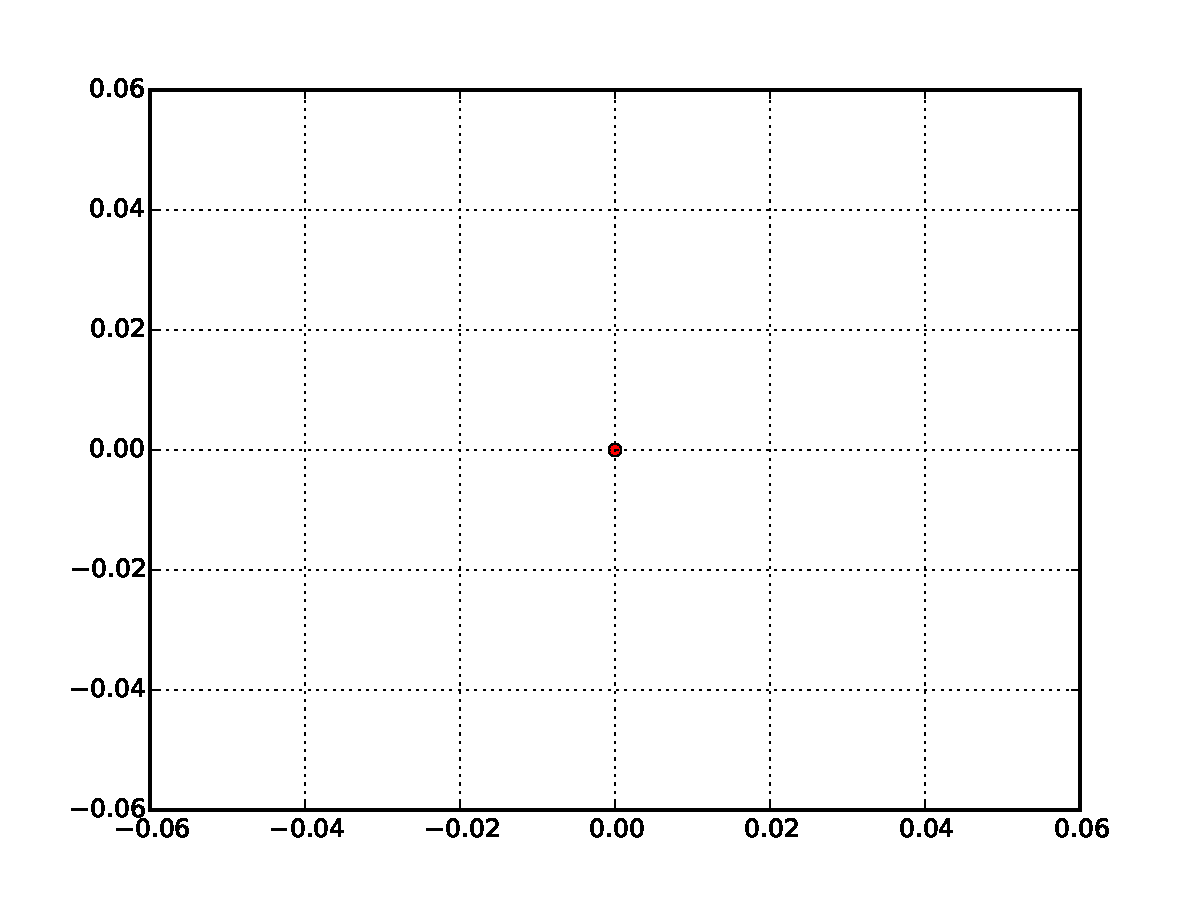
\includegraphics[width=0.7\linewidth]{figs/ex3_6_1.pdf}

\begin{verbatim}
x,y= symbols('x,y')
v= Matrix([x, y])
A= eye(2)

sols= solve(Eq(A*v, Matrix([0, 0])))[0] ## [{x: 0, y: 0}]
A.nullspace() ## Empty. 

plt.plot(sols[x], sols[y], 'ro')
plt.grid()
plt.savefig('figs/ex3_6_1.pdf')
\end{verbatim}

For $\mathbf{A}= \left[\begin{matrix}1 & 2\\2 & 4\end{matrix}\right]$ we need to
solve $\left[\begin{matrix}x + 2 y\\2 x + 4 y\end{matrix}\right] = \left[\begin{matrix}0\\0\end{matrix}\right]$.
Solution is $\left \{ x : - 2 y\right \}$ or $\left[\begin{matrix}-2\\1\end{matrix}\right]$.
Graphically, the nullspace is the vector passing by $\left[\begin{matrix}-2\\1\end{matrix}\right]$
as shown here below. In fact any point sitting on this line will make $\mathbf{Av = O}$.
\emph{E.g.} with $\mathbf{v} = [2\ -1]^T$ we have $\left[\begin{matrix}1 & 2\\2 & 4\end{matrix}\right] \left[\begin{matrix}2\\-1\end{matrix}\right] =
\left[\begin{matrix}0\\0\end{matrix}\right]$

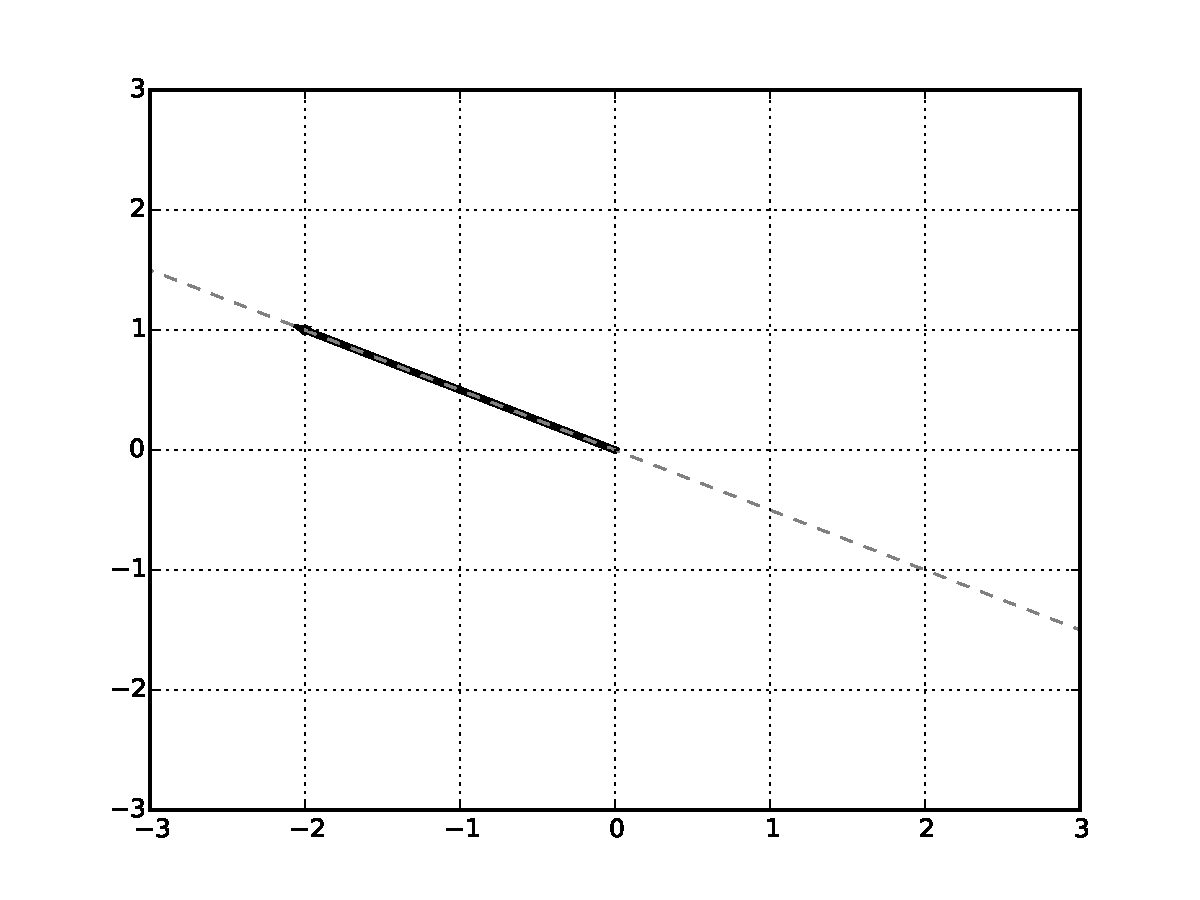
\includegraphics[width=0.7\linewidth]{figs/ex3_6_1b.pdf}

\begin{verbatim}
A= Matrix(2, 2, [1, 2, 2, 4])

sols= solve(Eq(A*v, zeros(A.rows, 1)))[0]
## Or simply
nsp= A.nullspace()[0]

plt.plot((0, nsp[0]*3), (0, nsp[1]*3))

plt.plot((-nsp[0]*3, nsp[0]*3), (-nsp[1]*3, nsp[1]*3), color= 'grey',
    linestyle= '--')
plt.arrow(0, 0, float(nsp[0]), float(nsp[1]), 'g', lw= 3)
plt.xlim(-3, 3)
plt.ylim(-3, 3)
plt.grid()
plt.savefig('figs/ex3_6_1b.pdf')
\end{verbatim}

For $\left[\begin{matrix}1 & 0\\1 & 2\\6 & 10\end{matrix}\right]$ we need to solve
$\left[\begin{matrix}x\\x + 2 y\\6 x + 10 y\end{matrix}\right] = \left[\begin{matrix}0\\0\\0\end{matrix}\right]$.
This is for $\left \{ x : 0, \quad y : 0\right \}$.

\begin{verbatim}
A= Matrix(3, 2, [1, 0, 1, 2, 6, 10])

sols= solve(Eq(A*v, zeros(A.rows, 1)))[0]
## Or
A.nullspace() # -> []
\end{verbatim}


For $\left[\begin{matrix}1 & 2\\3 & 4\\5 & 6\end{matrix}\right]$ we have
$\left[\begin{matrix}x + 2 y\\3 x + 4 y\\5 x + 6 y\end{matrix}\right] = \left[\begin{matrix}0\\0\\0\end{matrix}\right]$
solved only for $x= 0; y= 0$

\begin{verbatim}
A= Matrix(3, 2, [1, 2, 3, 4, 5, 6])
sols= solve(Eq(A*v, zeros(A.rows, 1)))[0]
\end{verbatim}

\subsubsection{Exercise 3.6.3}
%-----------------------------
Determine nullspace and nullity for
$\mathbf{A} = \left[\begin{matrix}1 & -2 & -3\\4 & -5 & -6\\7 & -8 & -9\end{matrix}\right]$.

The solution to 
$\left[\begin{matrix}x - 2 y - 3 z\\4 x - 5 y - 6 z\\7 x - 8 y - 9 z\end{matrix}\right] =
\left[\begin{matrix}0\\0\\0\end{matrix}\right]$.

is $\left \{ x : - z, \quad y : - 2 z\right \}$. Rearranged in vector form we have
$\left[\begin{matrix}x\\y\\z\end{matrix}\right] =
\left[\begin{matrix}-z\\-2z\\z\end{matrix}\right] =
z(\left[\begin{matrix}-1\\-2\\1\end{matrix}\right])
$ for $z$ being any real. Note therefore that the nullspace is the solution to the
linear system.

The nullity is the dimension of the nullspace. In this case only one vector makes
the nullspace, hence $nullity(\mathbf{A}) = 1$

\begin{verbatim}
A= Matrix([[1, -2, -3],
           [4, -5, -6],
           [7, -8, -9]])
x,y,z= symbols('x,y,z')
v= Matrix([x, y, z])
sols= solve(Eq(A*v, zeros(A.rows, 1)), x)[0]
v.subs(sols)
# Also
nsp= A.nullspace() # -> [[-1, -2, 1]]
nlty= len(nsp)     # -> 1
\end{verbatim}

For $\mathbf{A} = \left[\begin{matrix}2 & -2 & -2\\4 & -4 & -4\\8 & -8 & -8\end{matrix}\right]$
the linear systen to solve is
$\left[\begin{matrix}2 x - 2 y - 2 z\\4 x - 4 y - 4 z\\8 x - 8 y - 8 z\end{matrix}\right] =
\left[\begin{matrix}0\\0\\0\end{matrix}\right]$. Solved for $\left \{ x : y + z\right \}$.
Substituing the results in \textbf{v} we have the nullspace:

$
\mathbf{v_{sol}} = \left[\begin{matrix}x\\y\\z\end{matrix}\right] =
\left[\begin{matrix}y + z\\y\\z\end{matrix}\right] =
y(\left[\begin{matrix}1\\1\\0\end{matrix}\right]) + z(\left[\begin{matrix}1\\0\\1\end{matrix}\right])
$

The nullspace is made of two vectors $y(\left[\begin{matrix}1\\1\\0\end{matrix}\right]) + z(\left[\begin{matrix}1\\0\\1\end{matrix}\right])$
hence the nullity is 2. Note that $rank(\mathbf{A}) = 1$ consistent with $nullity(\mathbf{A}) + rank(\mathbf{A}) = n$

\begin{verbatim}
A= Matrix([[2, -2, -2],
           [4, -4, -4],
           [8, -8, -8]])
sols= solve(Eq(A*v, zeros(A.rows, 1)), x)
v.subs(sols)
# Equivalent to
y*Matrix([1,1,0]) + z*Matrix([1, 0, 1])
# Same as
nsp= A.nullspace()
nlty= len(nsp)
\end{verbatim}

This system
$\left[\begin{matrix}2 x + 9 y - 3 z\\5 x + 6 y - z\\9 x + 8 y - 9 z\end{matrix}\right] =
\left[\begin{matrix}0\\0\\0\end{matrix}\right]$
has solution only for $\left [ \left \{ x : 0, \quad y : 0, \quad z : 0\right \}\right ]$
hence the nullspace is the zero vector and the nullity is 0. In fact, the
dimension of the zero vector is zero.

\begin{verbatim}
A= Matrix([[2, 9, -3],
           [5, 6, -1],
           [9, 8, -9]])
sols= solve(Eq(A*v, zeros(A.rows, 1)))
nsp= A.nullspace() # -> []
nlty= len(nsp)     # -> 0
\end{verbatim}

Same as above for $\mathbf{A}= \left[\begin{matrix}-3 & 1 & -1\\2 & 5 & -7\\4 & 8 & -4\end{matrix}\right]$

\begin{verbatim}
A= Matrix([[-3, 1, -1],
           [2, 5, -7],
           [4, 8, -4]])
sols= solve(Eq(A*v, zeros(A.rows, 1)))
\end{verbatim}

\subsubsection{Exercise 3.6.4}
%-----------------------------

Determine the nullspace and nullity of
$\left[\begin{matrix}1 & 2 & 3 & 4 & 5 & 6 & 7\\
                     8 & 9 & 10 & 11 & 12 & 13 & 14\\
                     15 & 16 & 17 & 18 & 19 & 20 & 21\\
                     22 & 23 & 24 & 25 & 26 & 27 & 28\\
                     29 & 30 & 31 & 32 & 33 & 34 & 35\end{matrix}\right]$

Nullspace is
$
\left [ \left[\begin{matrix}1\\-2\\1\\0\\0\\0\\0\end{matrix}\right], \quad
        \left[\begin{matrix}2\\-3\\0\\1\\0\\0\\0\end{matrix}\right], \quad
        \left[\begin{matrix}3\\-4\\0\\0\\1\\0\\0\end{matrix}\right], \quad
        \left[\begin{matrix}4\\-5\\0\\0\\0\\1\\0\end{matrix}\right], \quad
        \left[\begin{matrix}5\\-6\\0\\0\\0\\0\\1\end{matrix}\right]\right ]
$ contaning five vectors, five is the nullity of \textbf{A}.

\begin{verbatim}
x1,x2,x3,x4,x5,x6,x7= symbols('x1:8')
A= Matrix(5, 7, range(1, 36))
sols= solve(Eq(A*v, zeros(A.rows, 1)))
v.subs(sols) # Nullspace. You could read out the nullspace vectors from here
nsp= A.nullspace()
nly= len(A) # 5
\end{verbatim}

\subsubsection{Exercise 3.6.5}
%-----------------------------

Determine bases for row, column and null space for
$\mathbf{A} = \left[\begin{matrix}1 & -4 & -9\\2 & 5 & -7\end{matrix}\right]$.

In other words, we need to find a set of \textbf{linearly independent} vectors such that
every vector in the given vector space (e.g. row space) is \textbf{linearly dependent} of these
vectors. Bases or coordinates are the basic building blocks to represent a vector
space.

To find a basis for the rows of a matrix (i.e. for this vector space) we need to
put the matrix un RREF. The rows of the RREF matrix are linearly independent. For
the rows in \textbf{A},
$\mathbf{A_{rref}} =
\left[\begin{matrix}1 & 0 & - \frac{73}{13}\\0 & 1 & \frac{11}{13}\end{matrix}\right] =
\left[\begin{matrix}13 & 0 & -73\\0 & 13 & 11\end{matrix}\right]$,

the rows of $\mathbf{A_{rref}}$ are the bases for the row space of $\mathbf{A}$.

The basis for the column vector can be obtained by looking at the leading 1s in
$A_{rref}$, these are $\left[\begin{matrix}1 & 0\\0 & 1\end{matrix}\right]$. \emph{
The same conclusion is reached by transposing \textbf{A} and repeating the reasoning
for the row space. Like \texttt{A.transpose().rref()}}

The basis for the nullspace is given by a nullspace itself \texttt{A.nullspace()}
which is $\left[\begin{matrix}\frac{73}{13}\\- \frac{11}{13}\\1\end{matrix}\right]$.
In this case the nullity is 1.

\begin{verbatim}
A= Matrix(2, 3, [1, -4, -9, 2, 5, -7])
B= Matrix(3, 2, [1, 3, 2, 5, -14, -37])
C= Matrix([[1, 3, -9, 5],
           [2, 6, 7, 1],
           [1, 3, -8, 1]])
rbasis= rref= A.rref()
cbasis= rref.A.transpose().rref()
nspbasis= A.nullspace()
\end{verbatim}

\subsubsection{Exercise 3.6.7}
%-----------------------------

Determine whether the following system have \emph{infinite}, \emph{unique}, or
\emph{no} solutions.

Without actually solving the system we can get the type of solution by looking
at the rank of coefficient matrix and augmented matrix:

\begin{itemize}
\item \textbf{Infinite solutions} $rank(\mathbf{A}) = rank(\mathbf{A_{augmented}}) < nrow(\mathbf{A})$
\item \textbf{Unique solution} $rank(\mathbf{A}) = rank(\mathbf{A_{augmented}}) = nrow(\mathbf{A})$
\item \textbf{No solution} $rank(\mathbf{A}) \neq rank(\mathbf{A_{augmented}})$
\end{itemize}


\begin{verbatim}
def numSolutions(A, b):
    rankA= A.rank()
    rankA_aug= Matrix(numpy.hstack([A, b])).rank()
    n= A.rows
    print 'nrow(A)= %s' %(n)
    print 'rank(A)= %s' %(rankA)
    print 'rank(A_aug)= %s' %(rankA_aug)
    if rankA == rankA_aug == n:
        return 'unique solution'
    elif rankA == rankA_aug < n:
        return 'oo solutions'
    elif rankA != rankA_aug:
        return 'no solutions'
    else:
        return None

A= Matrix([[1,2,3],
           [4,5,6],
           [7,8,9]])
b= Matrix([1,2,4])
numSolutions(A, b) # No solutions
\end{verbatim}

Consider the system

$$
A = \left[\begin{matrix}2x +& 5y & -3z & -7w\\
                        1x +& 1y & -4z & -8w\\
                        3x +& 4y & + 0z  & +1w \\
                        5x +& 21y & -1z & +3w
        \end{matrix}\right]
b= \left[\begin{matrix}0\\9\\6\\2\end{matrix}\right]
$$

It has a unique solution has showed here using ranks and verified by actually solving the
system. Solution are

$$
\left[\begin{matrix}x\\y\\z\\w\end{matrix}\right] =
\left[\begin{matrix}\frac{332}{117}\\
                    - \frac{545}{351}\\
                    - \frac{1091}{117}\\
                      \frac{1298}{351}
    \end{matrix}\right]
$$

\begin{verbatim}
A= Matrix([[2, 5, -3, -7],
           [1, 1, -4, -8],
           [3, 4, 0, 1],
           [5, 21, -1, 3]])
b= Matrix([0, 9, 6, 2])
numSolutions(A, b) ## Unique solution
nrow(A)= 4
rank(A)= 4
rank(A_aug)= 4

## Solve
xyzw_sols= A.solve(b)
\end{verbatim}

If we add a redundant row, the system is overdetermined and has infinite solutions:

$$
\mathbf{A}= \left[\begin{matrix}2 & 5 & -3 & -7\\1 & 1 & -4 & -8\\3 & 4 & 0 & 1\\5 & 21 & -1 & 3\\5 & 21 & -1 & 3\end{matrix}\right]
\mathbf{b}= \left[\begin{matrix}0\\9\\6\\2\\2\end{matrix}\right]
$$

Note also the exception thrown by \texttt{Matrix.solve} \textcolor{blue}{\texttt{
ValueError: For over-determined system, M, having more rows than columns,
try M.solve\_least\_squares(rhs).}}. Using least squares we get the
unique solution.

\begin{verbatim}
A= Matrix([[2, 5, -3, -7],
           [1, 1, -4, -8],
           [3, 4, 0, 1],
           [5, 21, -1, 3],
           [5, 21, -1, 3]])
b= Matrix([0, 9, 6, 2, 2])
numSolutions(A, b) ## 'oo solutions'
nrow(A)= 5
rank(A)= 4
rank(A_aug)= 4

A.solve(b) ## ValueError: For over-determined system

## Use linear least squares:
def linlsq(A, b):
    betas= (A.transpose() * A).inv() * A.transpose() * b
    return betas

## Same as sympy function:
linlsq(A, b)             ## [332/117], [-545/351], [-1091/117], [1298/351]
A.solve_least_squares(b) ## 
\end{verbatim}

\subsubsection{Exercise 3.6.8a}
%------------------------------

Test if the vectors \textbf{u} are in \emph{nullspace} of the corresponding
matrices:

\begin{itemize}
\item Get the nullspace of \textbf{A} by solving $\mathbf{Av= O}$
\item Test if \textbf{u} is a linear combination of the nullspace
\end{itemize}

To find the nullspace either use \sympy \texttt{Matrix.nullspace()} or solve the
system $\mathbf{Av= O}$ where \textbf{v} is a general vector of unknowns $[x_1\ x_2\ ...\ x_n]$.
Then, to extract the nullspace from the solution(s), substitute the solutions in
\textbf{v} and extract the coeffcients. For matrix

$$
\mathbf{A}= \left[\begin{matrix}1 & 1 & -1\\2 & -1 & 0\\5 & 2 & -3\end{matrix}\right]
$$

solve:

$$
\left[\begin{matrix}x_{1} + x_{2} - x_{3}\\2 x_{1} - x_{2}\\5 x_{1} + 2 x_{2} - 3 x_{3}\end{matrix}\right] = \left[\begin{matrix}0\\0\\0\end{matrix}\right]
$$

The solution are substituted in \textbf{v} and the coefficients extracted:

$$
sols= \left \{ x_{1} : \frac{x_{3}}{3}, \quad x_{2} : \frac{2 x_{3}}{3}\right \} =
\left[\begin{matrix}\frac{x_{3}}{3}\\\frac{2 x_{3}}{3}\\x_{3}\end{matrix}\right] =
x_3(\left[\begin{matrix}\frac{1}{3}\\\frac{2}{3}\\1\end{matrix}\right])
$$

So the nullspace is $x(\left[\begin{matrix}\frac{1}{3}\\\frac{2}{3}\\1\end{matrix}\right])$
for any real $x$.

\begin{verbatim}
u= Matrix([1, 2, 3])
A= Matrix([[1,1,-1], [2, -1, 0], [5, 2, -3]])

## Nullspace
x1,x2,x3= symbols('x1:4')
v= Matrix([x1, x2, x3])
sols= solve(Eq(A*v, zeros(A.rows, 1)))[0]
nsp= v.subs(sols) / x3

## Or simply
nsp= A.nullspace()
\end{verbatim}

Now, is the vector \textbf{u} part of the nullspace? See
\href{http://mathworld.wolfram.com/LinearlyDependentVectors.html}{LinearlyDependentVectors}
on Wolfram for different ways to test linear dependence between vectors.

\begin{verbatim}
## Test for linear dependence between u and nullspace vector:
detm= Matrix(2,2, [nsp.dot(nsp), nsp.dot(u),
             u.dot(nsp),   u.dot(u)]).det() ## == 0 -> u is in the nullspace

## Or test if 2xn matrix has rank < 2
Matrix(numpy.hstack([nsp, u])).transpose().rank() < 2 # rank<2. Vectors are lin.
                                                      # dep.
\end{verbatim}

Actually, the simple way is just to test:

$$
\mathbf{Au = O} =
\left[\begin{matrix}1 & 1 & -1\\2 & -1 & 0\\5 & 2 & -3\end{matrix}\right]
\left[\begin{matrix}1\\2\\3\end{matrix}\right] =
\left[\begin{matrix}0\\0\\0\end{matrix}\right]
$$

Since the nullspace is the set of vectors that transformed by \textbf{A} results
in the zero vector.

\begin{verbatim}
Eq(A*u, zeros(A.rows, 1)) ## True; u is in the nullspace of A
\end{verbatim}

\subsubsection{Exercise 3.6.8b}
%------------------------------

\begin{verbatim}
u= ones(3, 1)
B= Matrix(2, 3, [1, 4, -5,
                -7, 5,  2])
Eq(B*u, zeros(B.rows, 1)) # True: u is in the nullspace

## Or: extract nullspace from B and check if u is linearly dependent
nsp= B.nullspace()[0]
Matrix(numpy.hstack([nsp, u])).rank() < 2 # true: nullspace and u are lin dep
\end{verbatim}

\subsubsection{Exercise 3.6.8c}
%------------------------------

In case $\mathbf{u} = \left[\begin{matrix}1\\1\\1\end{matrix}\right];
\mathbf{C}= \left[\begin{matrix}1 & 3 & -9 & 5\\2 & 6 & 7 & 1\\1 & 3 & -8 & 1\end{matrix}\right]
$ dimensions are incompatible. Trying to compute \texttt{C*u} gives
\textcolor{blue}{\texttt{ShapeError: Matrices size mismatch.}} Consequently \textbf{u}
cannot be in the nullspace of \textbf{C}.

\begin{verbatim}
u= Matrix([2,1,5])
C= Matrix(2, 4, [1, 2, 3, 4,
                 5, 6, 7, 8])

Eq(C*u, zeros(C.rows, 1)) # ShapeError: Matrices size mismatch.
\end{verbatim}

\subsubsection{Exercise 3.6.8d}
%------------------------------

For $\mathbf{u}= \left[\begin{matrix}1\\3\\-4\\7\end{matrix}\right];
\mathbf{D}= \left[\begin{matrix}1 & -2 & 6 & 1\\3 & -6 & 7 & 8\\5 & 2 & 1 & 7\\1 & 6 & 3 & 2\end{matrix}\right];
\mathbf{Du} \neq \mathbf{O}$ \emph{I.e.} \textbf{u} is not in the nullspace. Note also
that $rank(\mathbf{D}) = nrow(\mathbf{D})$ and, consequently, $nullspace(\mathbf{D}) = null$.
Hence no vector is in the nullspace of \textbf{D}.


\begin{verbatim}
u= Matrix([1, 3, -4, 7])
D= Matrix([[1, -2, 6, 1],
           [3, -6, 7, 8],
           [5, 2, 1, 7],
           [1, 6, 3, 2]])

Eq(D*u, zeros(D.rows, 1)) # False, u not in nullspace

# Not also:
nsp= D.nullspace() # empty []
D.rank() == D.rows # Matrix is full rank
\end{verbatim}